\documentclass{beamer}
\usetheme[faculty=tw,language=dutch,framenumber,totalframenumber]{UniversiteitGent}
\usepackage{siunitx}
\usepackage{multicol}
\usepackage[]{hyperref}
\usepackage{soul}
\usepackage{tikz}
\usepackage{epstopdf}
\usepackage{tikz}
\usepackage{circuitikz}


\newcommand{\hcancel}[1]{%
    \tikz[baseline=(tocancel.base)]{
        \node[inner sep=0pt,outer sep=0pt] (tocancel) {#1};
        \draw[red] (tocancel.south west) -- (tocancel.north east);
        \draw[red]  (tocancel.north west) -- (tocancel.south east);
    }%
}%

\addtobeamertemplate{navigation symbols}{}{%
    \usebeamerfont{footline}%
    \usebeamercolor[fg]{footline}%
    \hspace{1em}%
    \insertframenumber/\inserttotalframenumber
}

\title{\textbf{Hardware Ontwerpproject}}
\subtitle{Indoor lokalisatie voor drones}
\author{Laurens Bogaert, Thomas Deckmyn \& Zeger Van de Vannet\\Groep 5}

\AtBeginSection[]{
  \begin{frame}
    \begin{multicols}{2}
    \frametitle{Inhoudstafel}
    \tableofcontents[currentsection]
  \end{multicols}
  \end{frame}
}

\usepackage{pifont}


\begin{document}

\begin{frame}
  \titlepage
\end{frame}

\section{Inleiding}
\subsection{Situering}
  \begin{frame}
    \frametitle{Situering}
    GPS:
    \begin{itemize}
        \item Niet voor binnen
        \item Onnauwkeurig (3 m)
        \item Hoogtemeting beperkt
    \end{itemize}
    Toepassing:
     \begin{itemize}
        \item Autonoom vliegen
    \end{itemize}   
  \end{frame}
  \begin{frame}
  \frametitle{Oplossing}
   \begin{columns}
    \begin{column}{0.5\textwidth}
  	\begin{itemize}
  		\item Afstandsbepaling
  		\item Communicatie
  	\end{itemize} 
    \end{column}
    \begin{column}{0.5\textwidth}
  	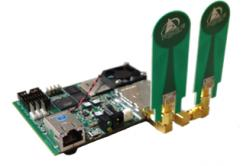
\includegraphics[width=\textwidth]{images/Pulson400UWB.jpg}
    \end{column}
    \end{columns}
  \end{frame} 
  \begin{frame}
    \frametitle{Situering}
    3 onderdelen:
    \begin{itemize}
      \item PCB + Controller
      \item Algoritmes
      \item Antenne
    \end{itemize}
  \end{frame}
\subsection{Planning}
  \begin{frame}
    \frametitle{Planning}
    \begin{tabular}{|l | l | l|}
      \hline
      Week & Titel & Status\\
      \hline
      1 & Toekenning onderwerp & \checkmark\\
      2 & Literatuurstudie \& $1^{ste}$ algoritme & \checkmark\\
      3 & Kennismaking ADS \& $2^{de}$ algoritme & \checkmark\\
      4 - 6 & Antenne design (L \& T) \& PCB-ontwerp (Z) & \checkmark \\
      7 & Afwerking $2^{de}$ algoritme \& Fabricage Antenne (T) & \checkmark \\
       & Vergelijking Algoritmes & \checkmark\\
      8 & Uitmeten Antenne  & \checkmark \\
      \hline
    \end{tabular}
  \end{frame}
  
    \begin{frame}
    \frametitle{Planning}
    \begin{tabular}{|l | l | l|}
      \hline
      Week & Titel & Status\\
      \hline
      Paas 1 \& 2 & Implementatie microcontroller & \checkmark\\
      9 & Bestukking PCB  & \checkmark\\
      10 & Afwerken Implementaties  & \checkmark\\
      11 & Afwerken (debuggen) + verslag schrijven & \checkmark \\
      12 & Afwerken (debuggen + synthese) + presentatie & \checkmark \\
      \hline
    \end{tabular}
  \end{frame}

\section{PCB Design}
\subsection{Onderdelen}
  \begin{frame}
    \frametitle{Vereisten}
    \begin{itemize}
      \item Microcontroller: verwerking van metingen tot positie
      \item Accelerometer:
      \begin{itemize}
      	\item Preciezere positiebepaling
      	\item Dynamic Power Management
      \end{itemize}
    \end{itemize}
  \end{frame}
  \begin{frame}
  	\frametitle{EMC}
      \begin{columns}[t]
        \begin{column}[T]{.5\textwidth}
          \begin{itemize}
            \item Volledig grondvlak
            \item ESD bescherming: Zener diodes
          \end{itemize}
        \end{column}
        \begin{column}[T]{.5\textwidth}
          \centering
          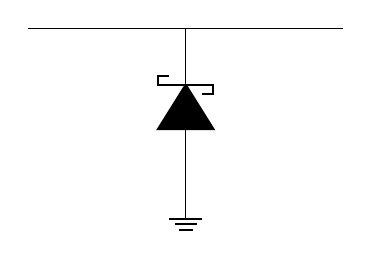
\begin{tikzpicture}
            \node [ground] {};
            \draw (0,0) to[sD*] (0,2);
            \draw (-2,2) -- (2,2);
          \end{tikzpicture}
        \end{column}
      \end{columns}
  \end{frame}
  \begin{frame}
    \begin{figure}
      \begin{center}
        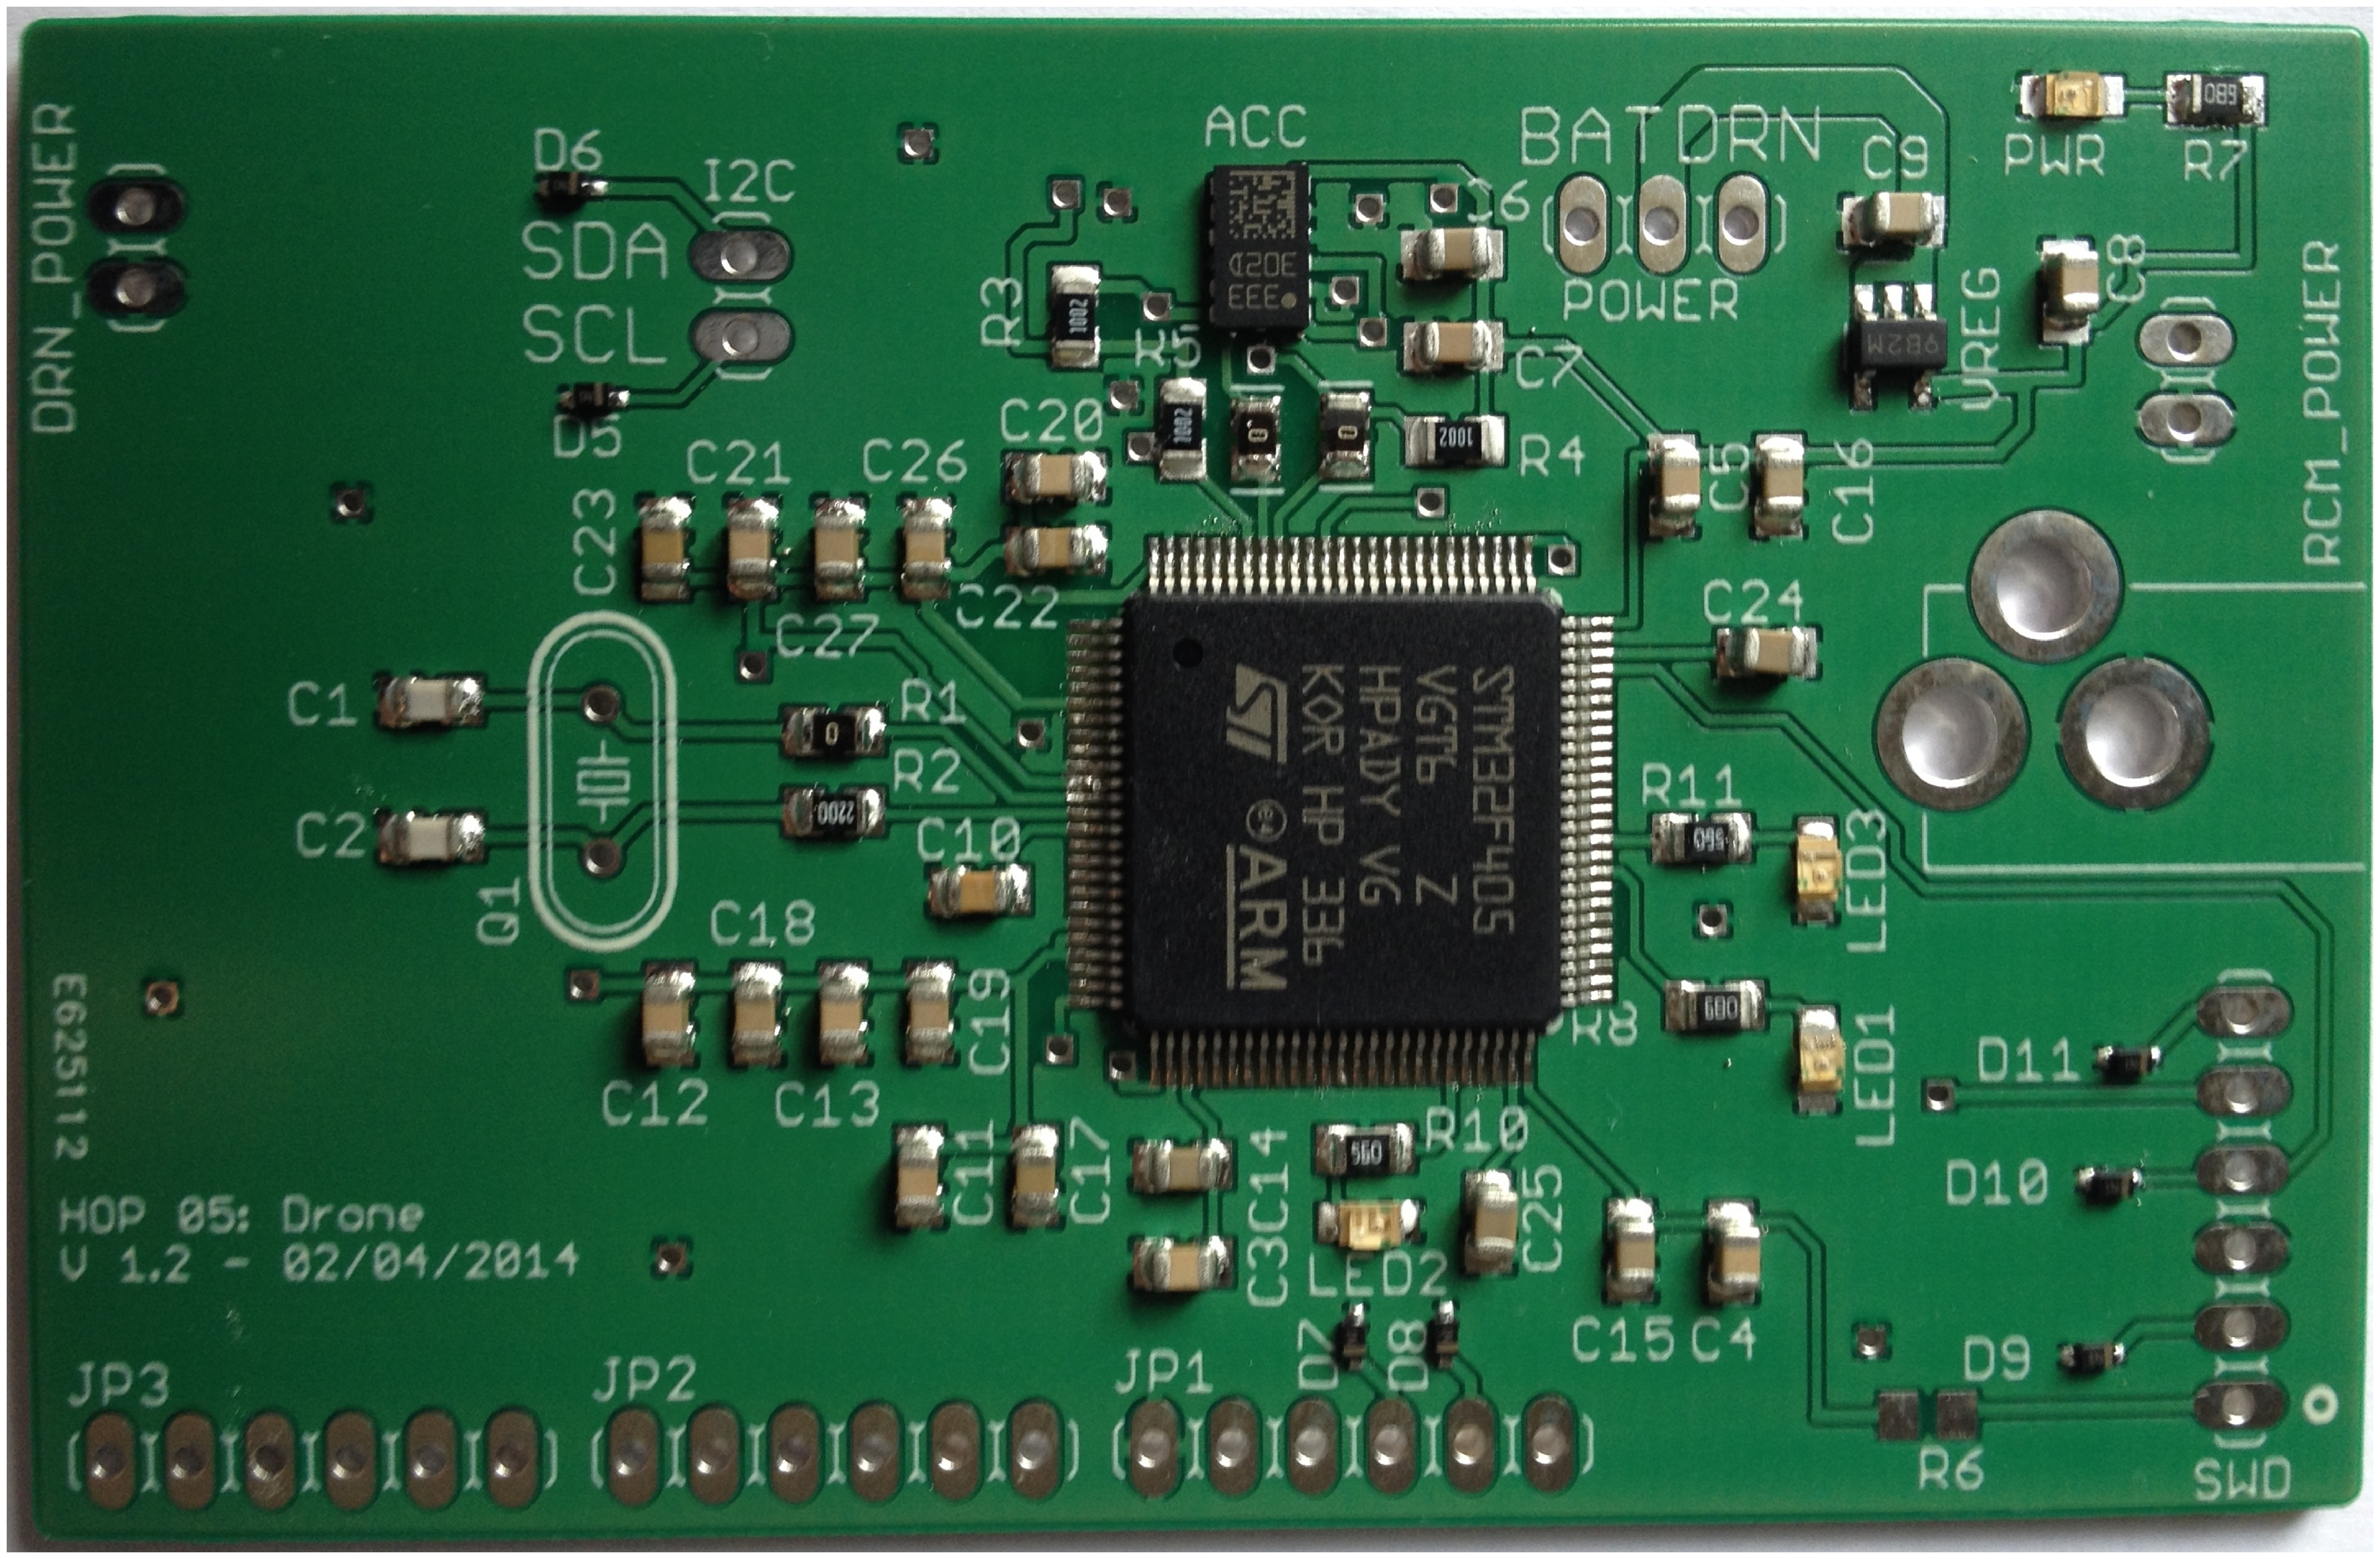
\includegraphics[width=\textwidth]{images/final.eps}
      \end{center}
    \end{figure}
  \end{frame}
\section{Algoritmes}
\subsection{Ankers}
  \begin{frame}
    \frametitle{Opstelling}
    \begin{figure}
      \begin{center}
        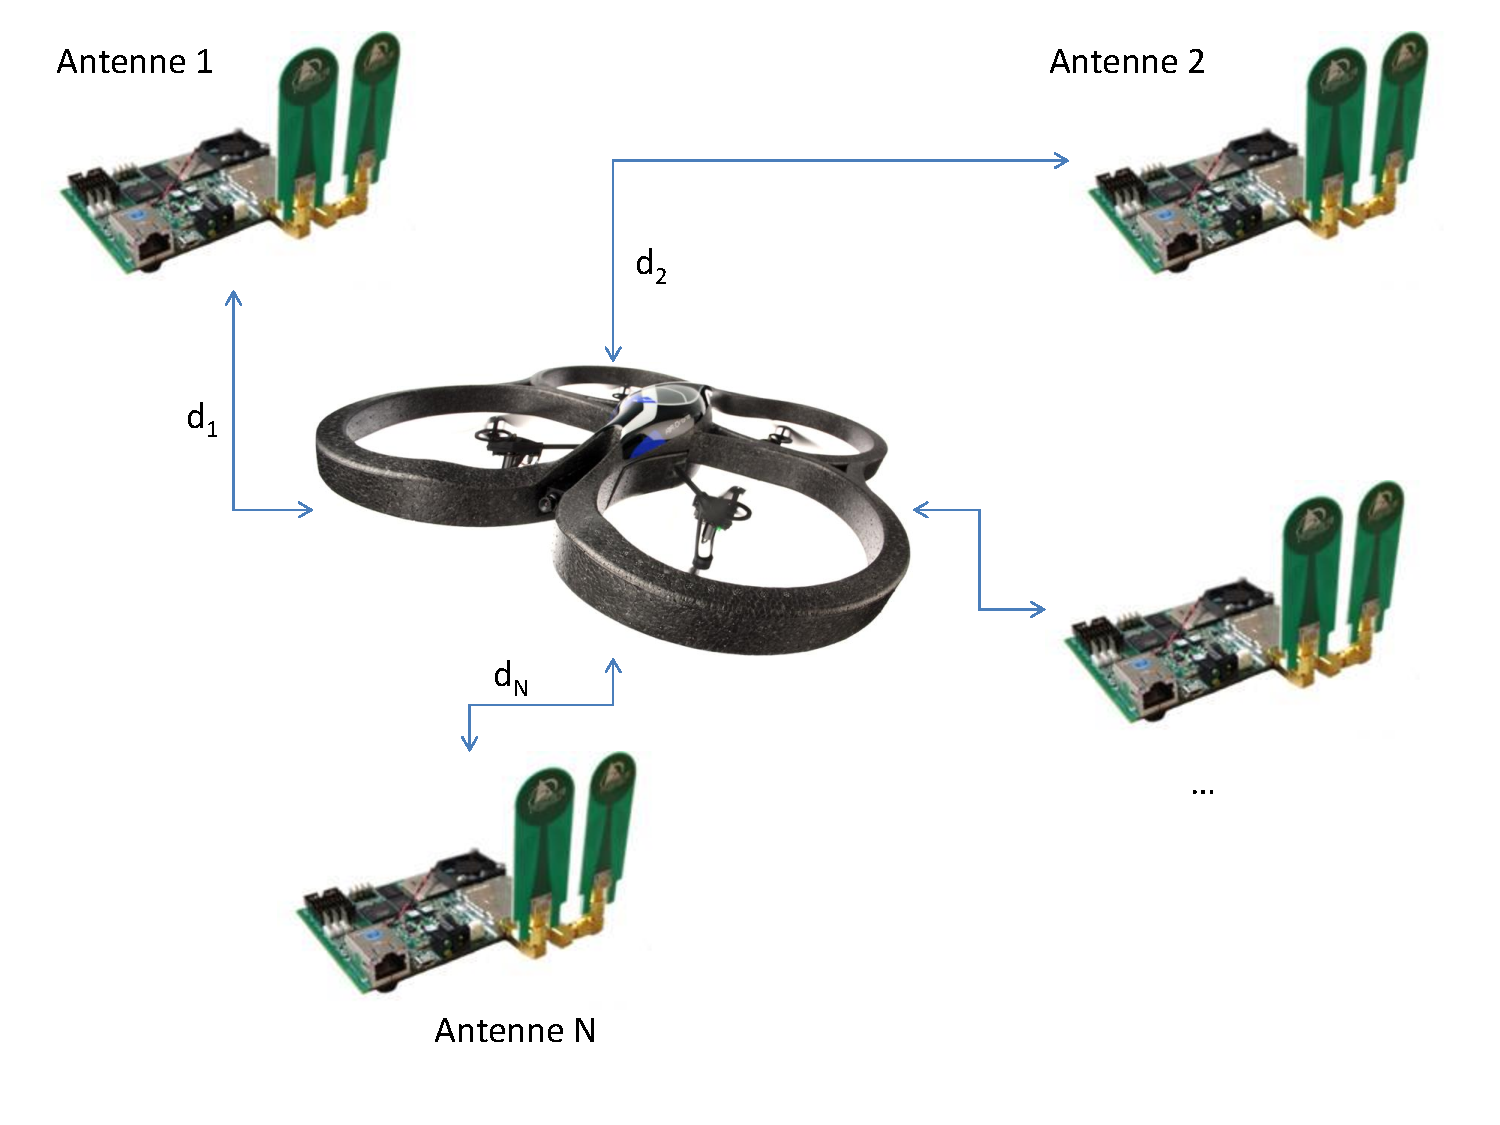
\includegraphics[width=.8\textwidth]{images/opstelling.pdf}
      \end{center}
    \end{figure}
  \end{frame}
  
  \begin{frame}
    \frametitle{Ankers}
    \begin{itemize}
      \item Gekende positie
      \item Afstand via pulsen $\Rightarrow$ UWB
      \item Meetruis
    \end{itemize}
    \begin{figure}
      \begin{center}
        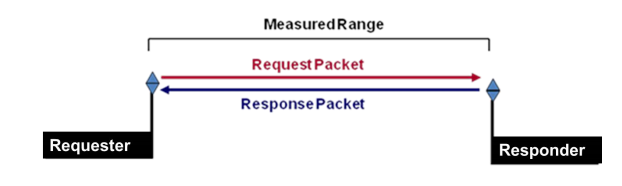
\includegraphics[width=.8\textwidth]{images/DME.png}
      \end{center}
    \end{figure}
  \end{frame}
\subsection{Lokalisatie Algoritme}
  \begin{frame}
    \frametitle{Algoritmes}
    \begin{itemize}
      \item Least Squares
      \item Kalman 
    \end{itemize}
  \end{frame}
  \begin{frame}
    \frametitle{Least Squares}
    \begin{itemize}
      \item Geen geheugen
        \begin{itemize}
          \item Geen invloed van het verleden
        \end{itemize}
    \end{itemize}
      \begin{figure}
      \centering
        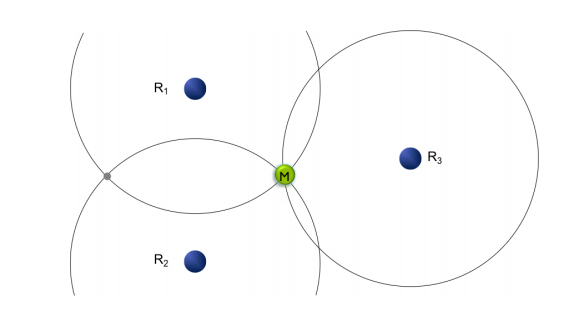
\includegraphics[width=.5\textwidth]{images/ranging.png}
    \end{figure}
  \end{frame}
  \begin{frame}
  \frametitle{Wat bij overdimensionering?}

    \begin{itemize}
    \item Laat NLOS metingen vallen
    \item Minimaliseer de gemiddelde kwadratische fout
    \end{itemize}
          \begin{figure}
      \centering
        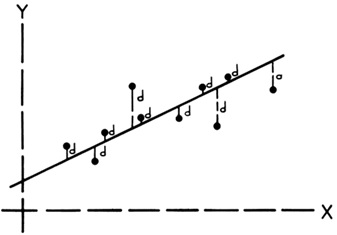
\includegraphics[width=.5\textwidth]{images/LMS.jpg}
    \end{figure}
  \end{frame}
  \begin{frame}
    \frametitle{Kalman Filter}
    \begin{itemize}
      \item Geheugen $\Rightarrow$ matrices
      \item Bewegingsvrijheid van de drone is beperkt
      \item 2 onderdelen:
        \begin{itemize}
          \item Voorspellen
          \item Meten en updaten
        \end{itemize}
    \end{itemize}
  \end{frame}
  \begin{frame}
    \frametitle{Uitbreiden Kalman Filter}
    \begin{itemize}
      \item Extra Sensoren (Sensor Fusion)
        \begin{itemize}
          \item Accelerometer
          \item Gyroscoop
          \item Hoogtemeter
          \item \ldots
        \end{itemize}
      \item Doel: nauwkeuriger volgen
    \end{itemize}
  \end{frame}
\subsection{Resultaten}
  \begin{frame}
    \frametitle{Resultaten: Simulaties}
    \begin{columns}[c]
      \begin{column}{.5\textwidth}
        \begin{figure}
          \begin{center}
            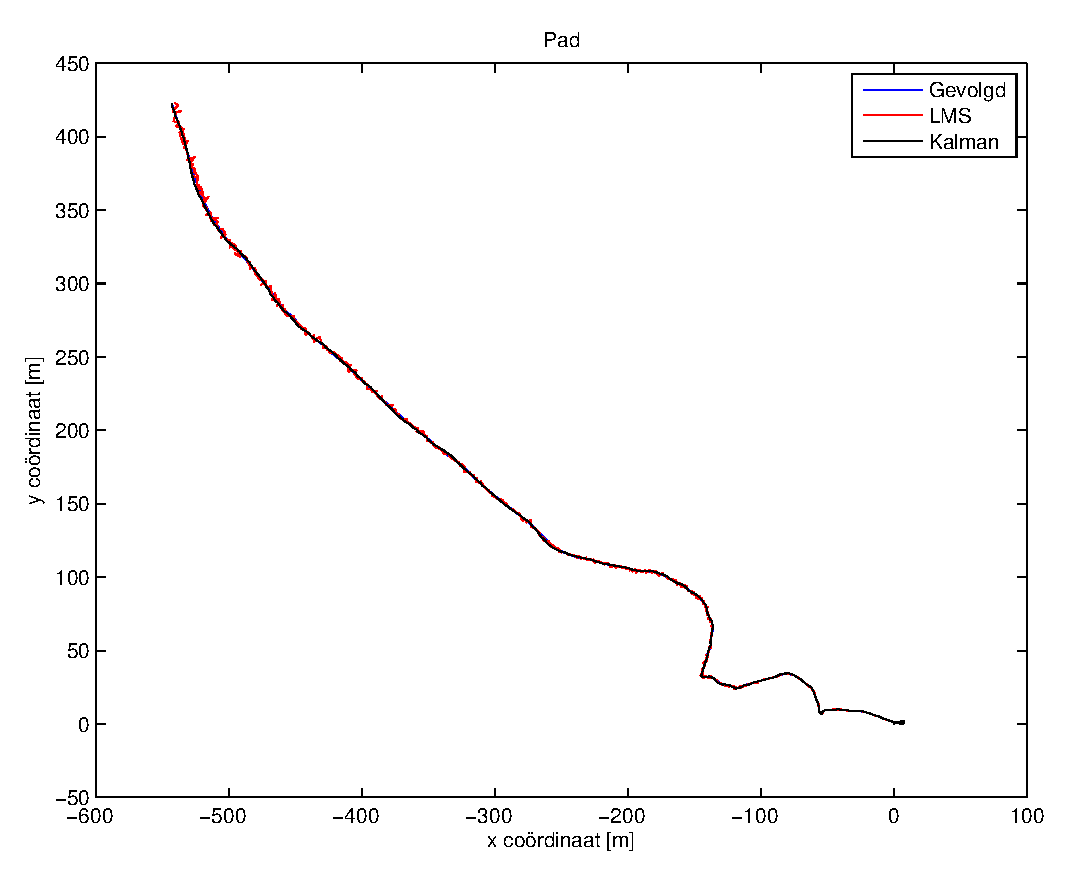
\includegraphics[width=\linewidth]{images/simulatie_pad.eps}
          \end{center}
        \end{figure}
      \end{column}
      \begin{column}{.5\textwidth}
        \begin{figure}
          \begin{center}
            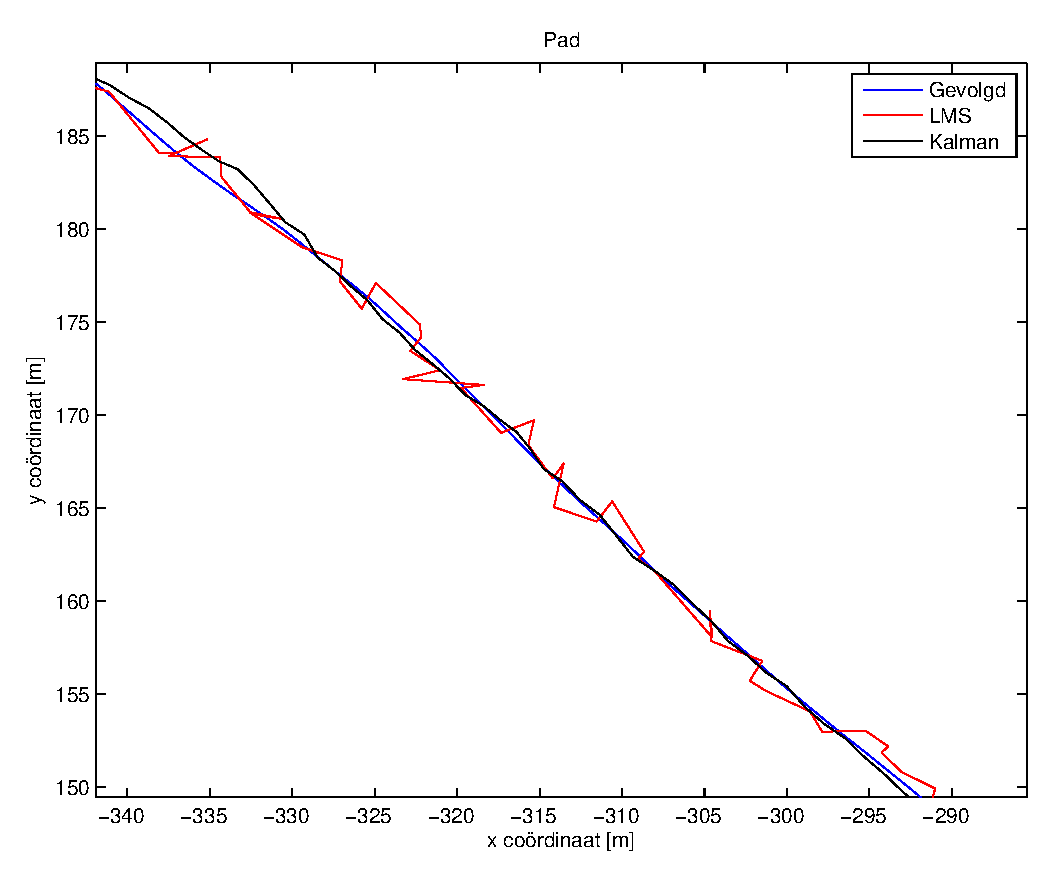
\includegraphics[width=\linewidth]{images/simulatie_pad_zoom.eps}
          \end{center}
        \end{figure}
      \end{column}
    \end{columns}
  \end{frame}
  
  \begin{frame}
    \frametitle{Resultaten: Simulaties}
    \begin{columns}[c]
  \begin{column}{0.5\textwidth}
    \begin{itemize}
      \item Gemiddelde kwadratische fout
      \end{itemize}
      \begin{equation*}
      \begin{split}
MSE = \dfrac{1}{3}((x_{real}-x_{est})^2+\\(y_{real}-y_{est})^2+\\(z_{real}-z_{est})^2 )
\end{split}
\end{equation*}
\begin{itemize}
      \item 90-ste percentiel
    \end{itemize}
    \end{column}

    \begin{column}{0.5\textwidth}
    \begin{figure}
      \begin{center}
        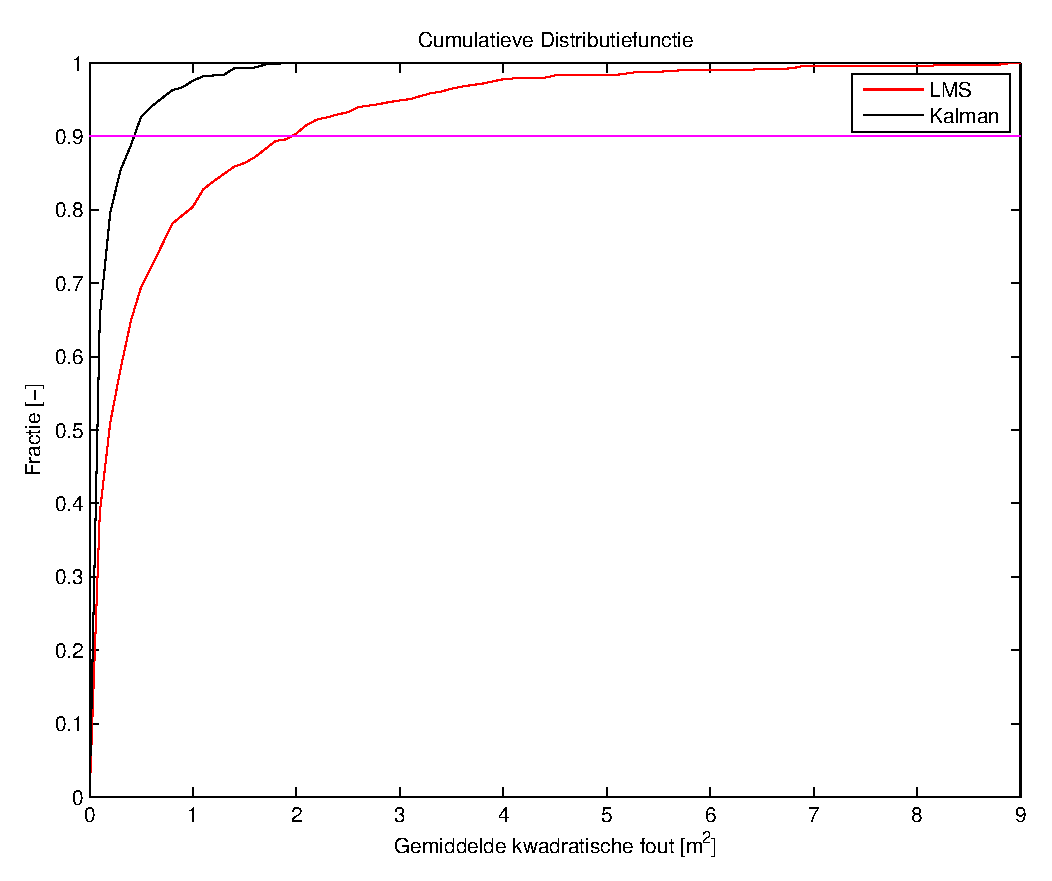
\includegraphics[width=1\linewidth]{images/simulatie_cumulatief.eps}
      \end{center}
    \end{figure}
    \end{column}
    \end{columns}

  \end{frame}
  
  \begin{frame}
    \frametitle{Least Squares vs. Kalman Filter}
    \begin{center}
    \begin{tabular}{|l|l|}
      \hline
      Least Squares & Kalman Filter \\
      \hline
      (+) Eenvoudiger & (-) Complexer \\
      (-) Ruwere schatting & (+) Nauwkeuriger \\
      \hline
    \end{tabular}
    \end{center}
  \end{frame}

  \addtocontents{toc}{\newpage}

\section{Microcontroller}
\subsection{Algemeen}
\begin{frame}
\begin{itemize}
\frametitle{Algemeen}
\item Matlab naar microcontroller
\item Refresh rate: $\pm$ 3 Hz
\begin{itemize}
\item Te laag voor autonoom vliegen
\end{itemize}
\end{itemize}
\end{frame}
\begin{frame}
\frametitle{LOS vs. NLOS: Rise Time}
 \begin{figure}
      \begin{center}
        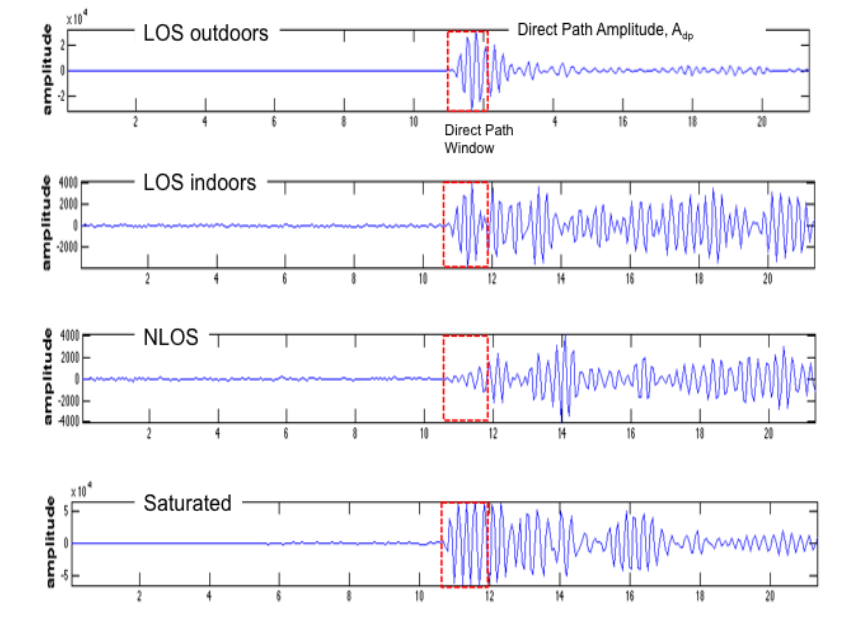
\includegraphics[width=0.7\linewidth]{images/NLOS.png}
      \end{center}
    \end{figure}
\end{frame}



\subsection{Problemen}
\begin{frame}
\frametitle{Problemen: 3D nauwkeurigheid}
\begin{itemize}
\item Matlab: goede spreiding in de 3D ruimte
\item Praktijk: kleinere z-spreiding ankers
\begin{itemize}
\item Lagere nauwkeurigheid in de z-richting
\end{itemize}
\end{itemize}
\end{frame}
\begin{frame}
\frametitle{Problemen: Gaussiaanse beweging}
\begin{itemize}
\item Kalman is gebaseerd op Gaussiaanse bewegings- en ruismodellen
\begin{itemize}
\item Te scherpe bochten 
\end{itemize}
\end{itemize}
\end{frame}
\subsection{Uitbreidingen}
\begin{frame}
\frametitle{Eventuele uitbreiding}
Kalman tunen via parameters:
\begin{itemize}
\item bewegingsvariantie
\item ruisvariantie
\item ...
\end{itemize}

Voorstel:
Model afhankelijk van type beweging\\
\begin{itemize}
\item parallelle filterbank
\end{itemize}
\end{frame}

\begin{frame}
\frametitle{Kalman Filterbank}
Parallelle filterbank:
\begin{itemize}

\item Stilstaan
\item Traag bewegen
\item Snel bewegen
\end{itemize}

Geef verschillende gewichten

\end{frame}
\section{UWB Antenne}
\subsection{Referentie}
  \begin{frame}
  \frametitle{Referentie}
  \begin{columns}[c]
  \begin{column}{0.5\textwidth}
    \begin{itemize}
      \item BroadSpec\texttrademark  UWB Antenne 
      \item Dipool: omni in azimuth
      \item Ontwerpsparameters:
      \begin{itemize}
        \item $\SI{3.1}{\giga\hertz}$ - $\SI{5.3}{\giga\hertz}$
        \item Gain nominaal $\approx \SI{3}{\decibel}$ 
        \item Lineaire fase respons
        \item Effici\"entie $\approx$ 90\%
      \end{itemize}
    \end{itemize}
    \end{column}

    \begin{column}{0.5\textwidth}
    \centering
      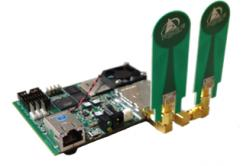
\includegraphics[width=0.7\textwidth]{images/Pulson400UWB.jpg}
    \end{column}
    \end{columns}
  \end{frame}


  \begin{frame}
  \frametitle{Ontwerp UWB Antenne}
  \begin{itemize}
    \item Start: Rechthoekige Patch Antenne
      \begin{itemize}
        \item Lengte: Resonantie frequentie $f_0 = \SI{4.2}{\giga\hertz}$
              \begin{align}  L = \frac{c}{2 f_r \sqrt{\epsilon_r}}  \nonumber \end{align}
        \item Breedte: \begin{align} \text{Uitgestraald vermogen} \nonumber & \implies \text{Resonantie weerstand} \downarrow \\ & \implies \text{Bandbreedte} \uparrow, \text{Effici\"entie} \uparrow \nonumber \end{align}

      \end{itemize}
    \item Dimensies drone! $\implies$ Andere manier BW $\uparrow$ 
    \end{itemize}
  \end{frame}

  \begin{frame}
  \frametitle{Ontwerp UWB Antenne}
  
  \begin{columns}[c]
  \begin{column}{0.5\textwidth}
    \begin{itemize}
      \item Toevoegen \textit{Trap} $\implies$ BW $\uparrow$
      \item Partieel grondvlak
      \begin{itemize}
        \item Optimaliseren dimensies \begin{align} & \implies \text{Vlakke } S_{11} \nonumber \\ & \implies \text{Lineaire fase} \nonumber \end{align}
      \end{itemize}

    \end{itemize}
  \end{column}

  \begin{column}{0.5\textwidth}
  \centering
    
\includegraphics[width=0.7\textwidth]{images/patch_stairs.pdf}
  \end{column}
  \end{columns}
  \end{frame}

\subsection{Simulatie}
  \begin{frame}
  \frametitle{ADS Simulatie}
    \begin{columns}[c]
      \begin{column}{0.5\textwidth}
      \begin{itemize}
        \item $S_{11} < \SI{-10}{\decibel}$: \\ $\SI{3.1}{\giga\hertz}$ - $\SI{6.7}{\giga\hertz}$
      \end{itemize}
        \begin{figure}
          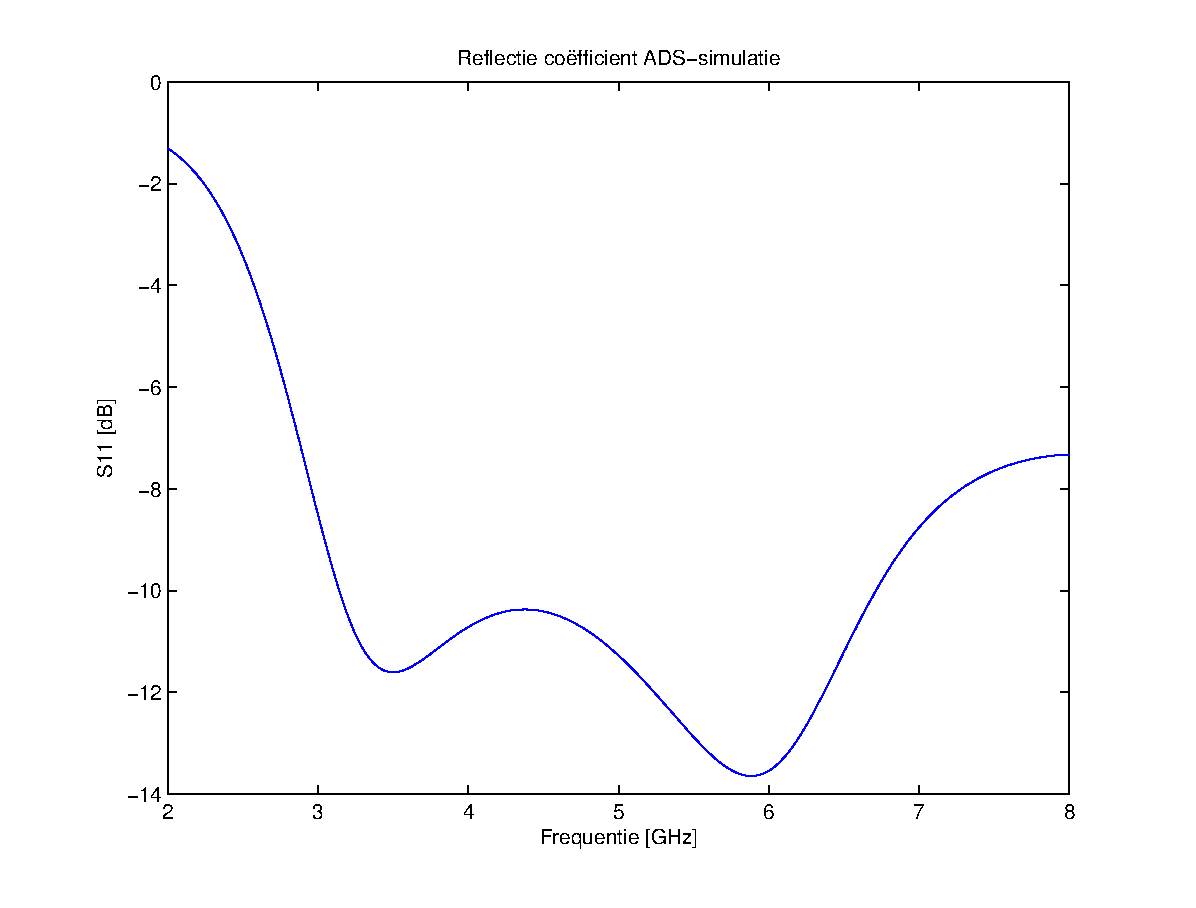
\includegraphics[width=\textwidth]{images/S11_ADS_sim.eps}
        \end{figure}

      \end{column}

      \begin{column}{0.5\textwidth}
      \begin{itemize}
        \item Lineaire fase respons: \\ OK
      \end{itemize}
        \begin{figure}
          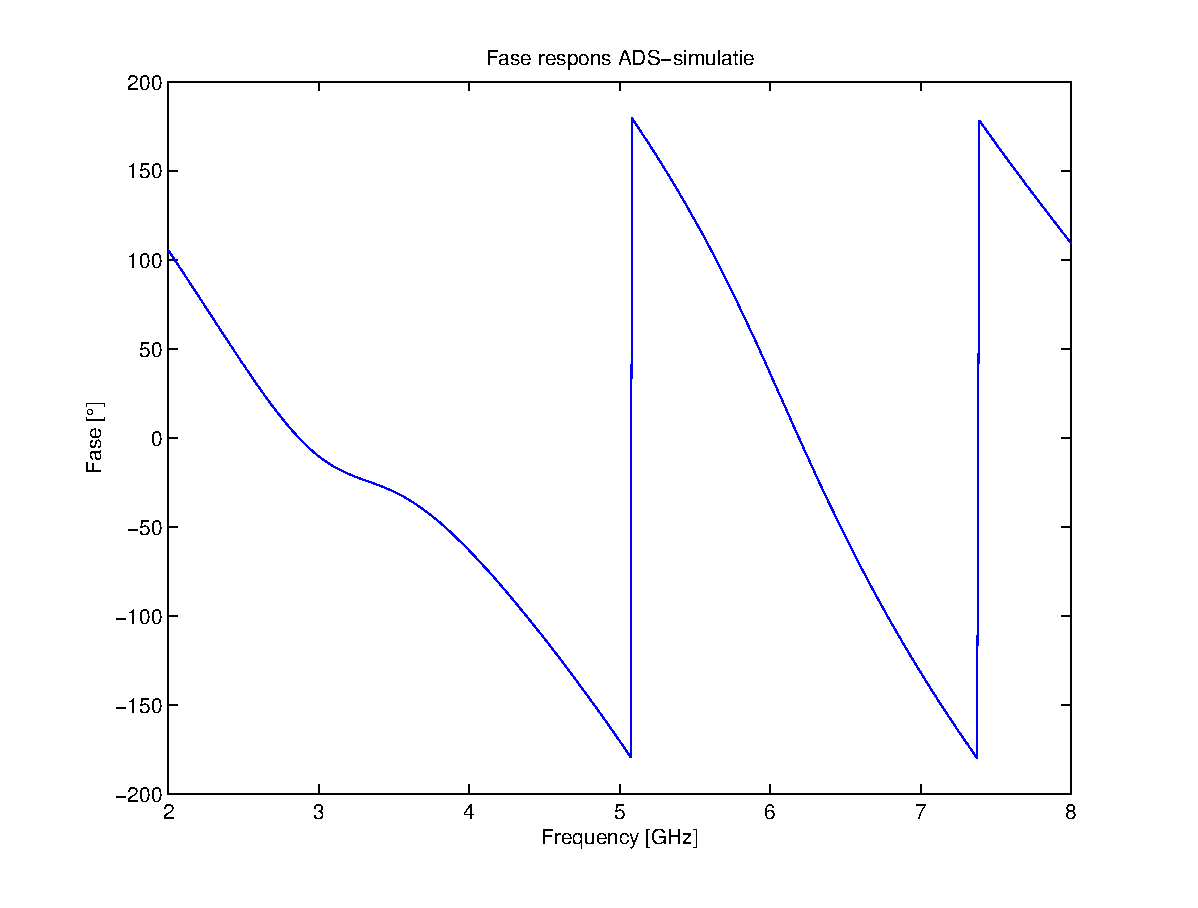
\includegraphics[width=\textwidth]{images/fase_respons_ADS_sim.eps}
        \end{figure}
      \end{column}
    \end{columns}
  \end{frame}

  \begin{frame}
  \frametitle{ADS Simulatie}
    \begin{columns}[c]
      \begin{column}{0.5\textwidth}
      \begin{itemize}
        \item Effici\"entie 50\% - 96\% in gewenste band
      \end{itemize}
        \begin{figure}
          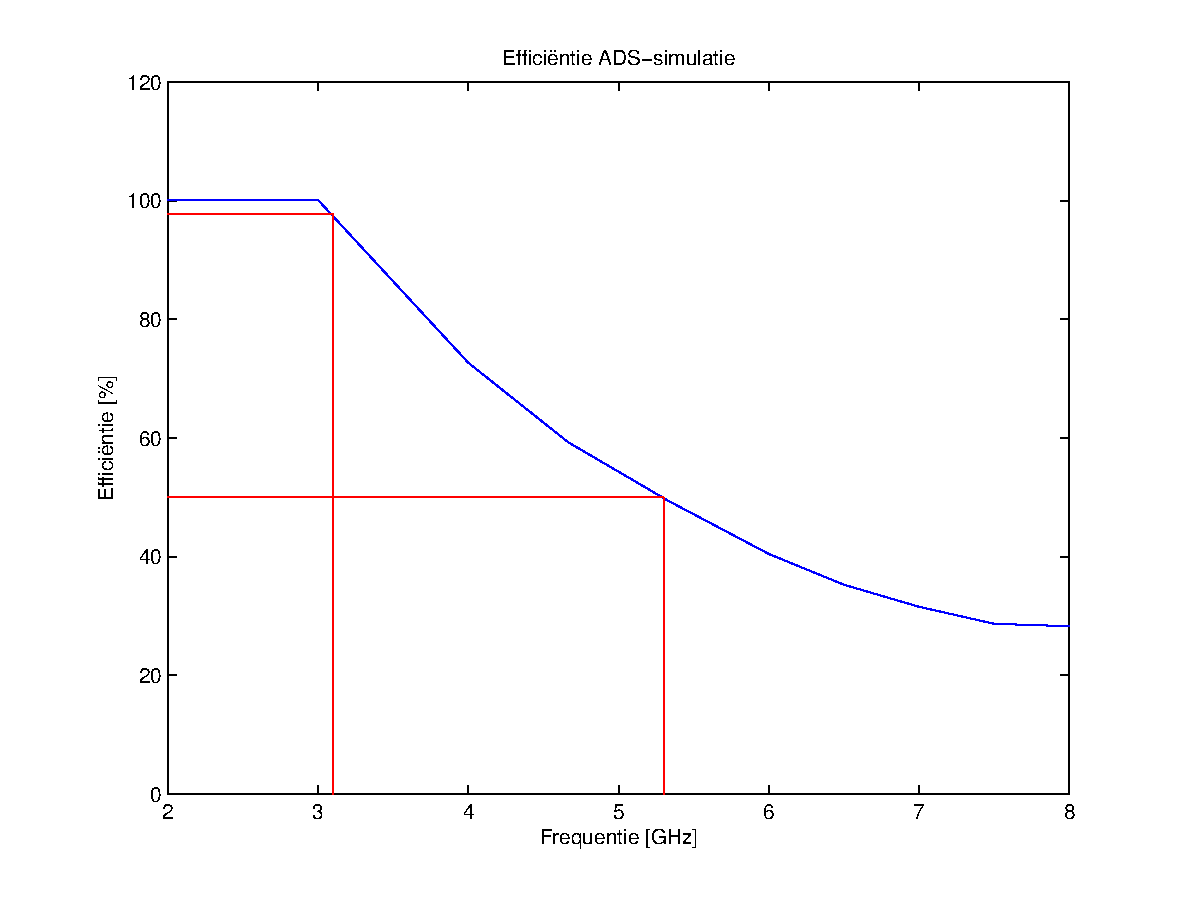
\includegraphics[width=\textwidth]{images/eff_ADS_sim.eps}
        \end{figure}

      \end{column}

      \begin{column}{0.5\textwidth}
      \begin{itemize}
        \item Gain $\approx \SI{3}{\decibel}$ in gewenste band 
      \end{itemize}
        \begin{figure}
          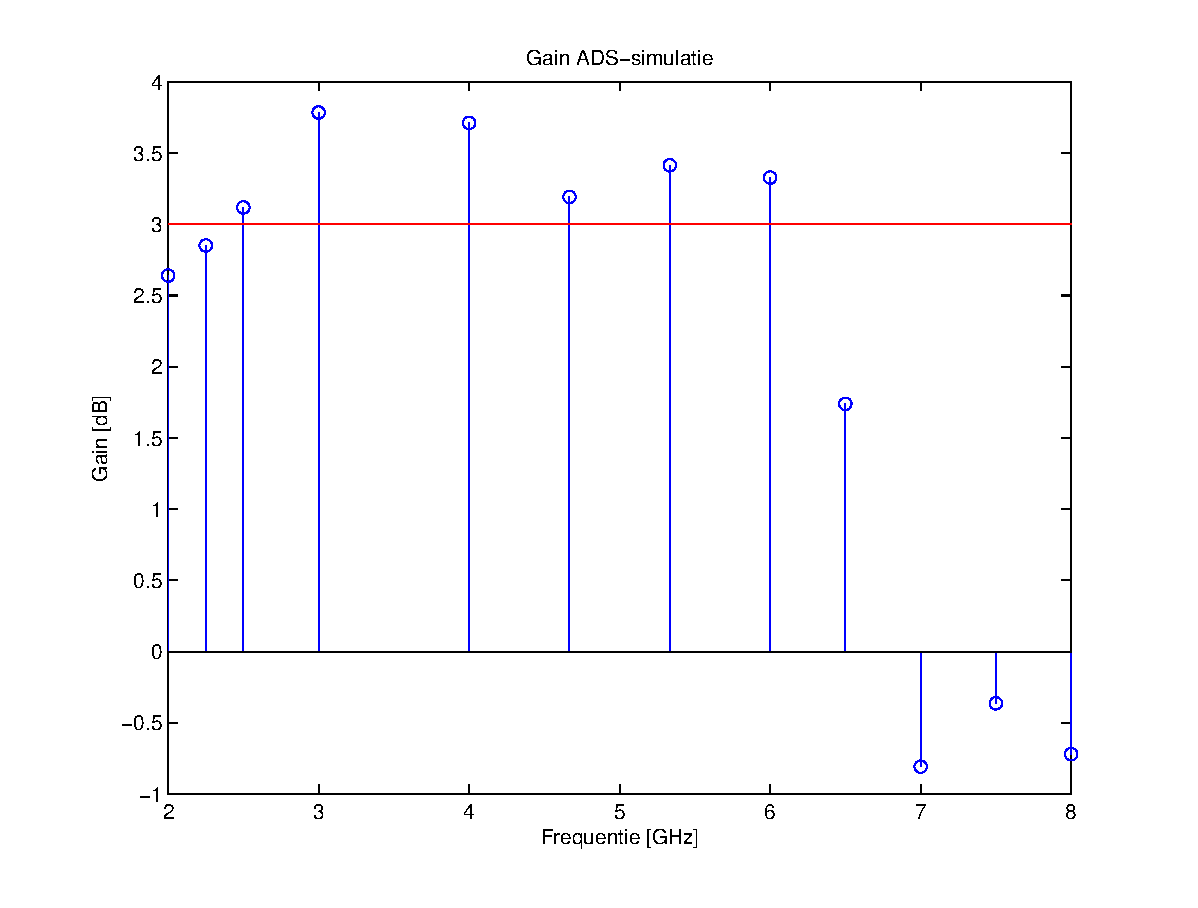
\includegraphics[width=\textwidth]{images/gain_ADS_sim.eps}
        \end{figure}
      \end{column}
    \end{columns}
  \end{frame}

\subsection{Prototype}
  \begin{frame}
  \frametitle{Prototype}
    \begin{itemize}
      \item Manuele fabricatie 
      \begin{itemize}
      	\item Foute alignatie t.o.v. grondvlak
      	\item Prototype versie 2.0
      \end{itemize} 
    \end{itemize}
    \begin{columns}[c]
    \begin{column}{0.5\textwidth}
      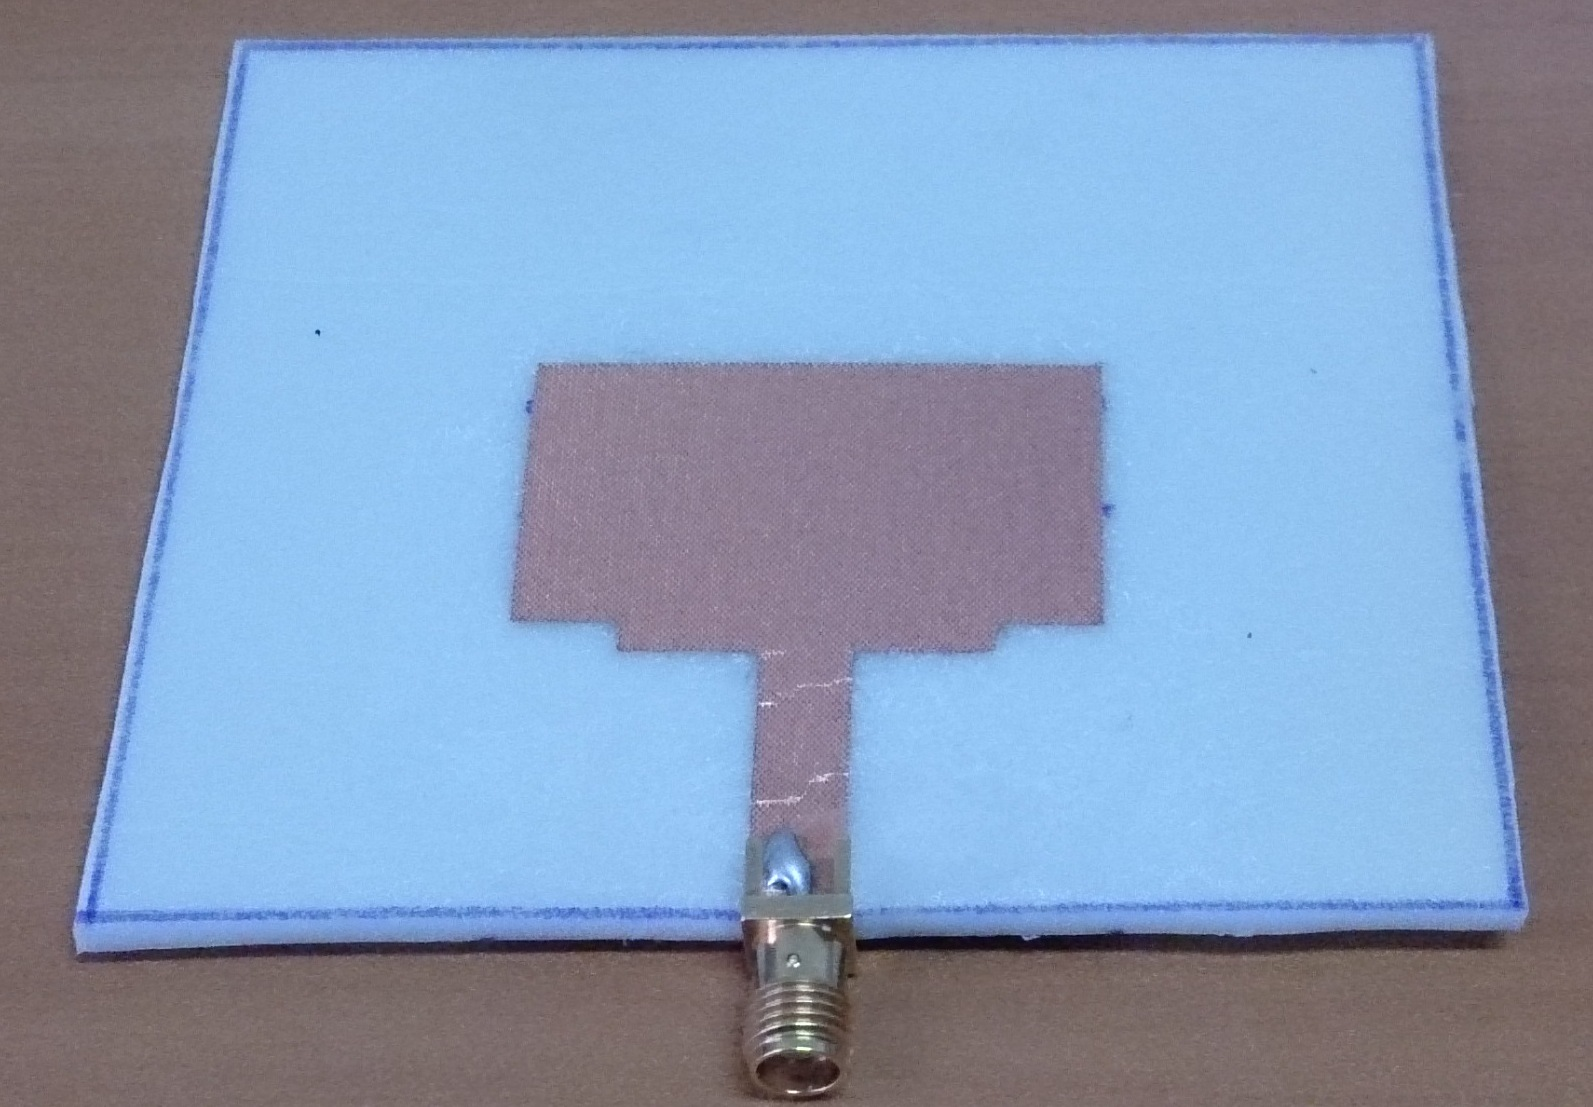
\includegraphics[width=\textwidth, height=0.75\textwidth]{images/patch_proto_front.jpg}
    \end{column}%
    \begin{column}{0.5\textwidth}
      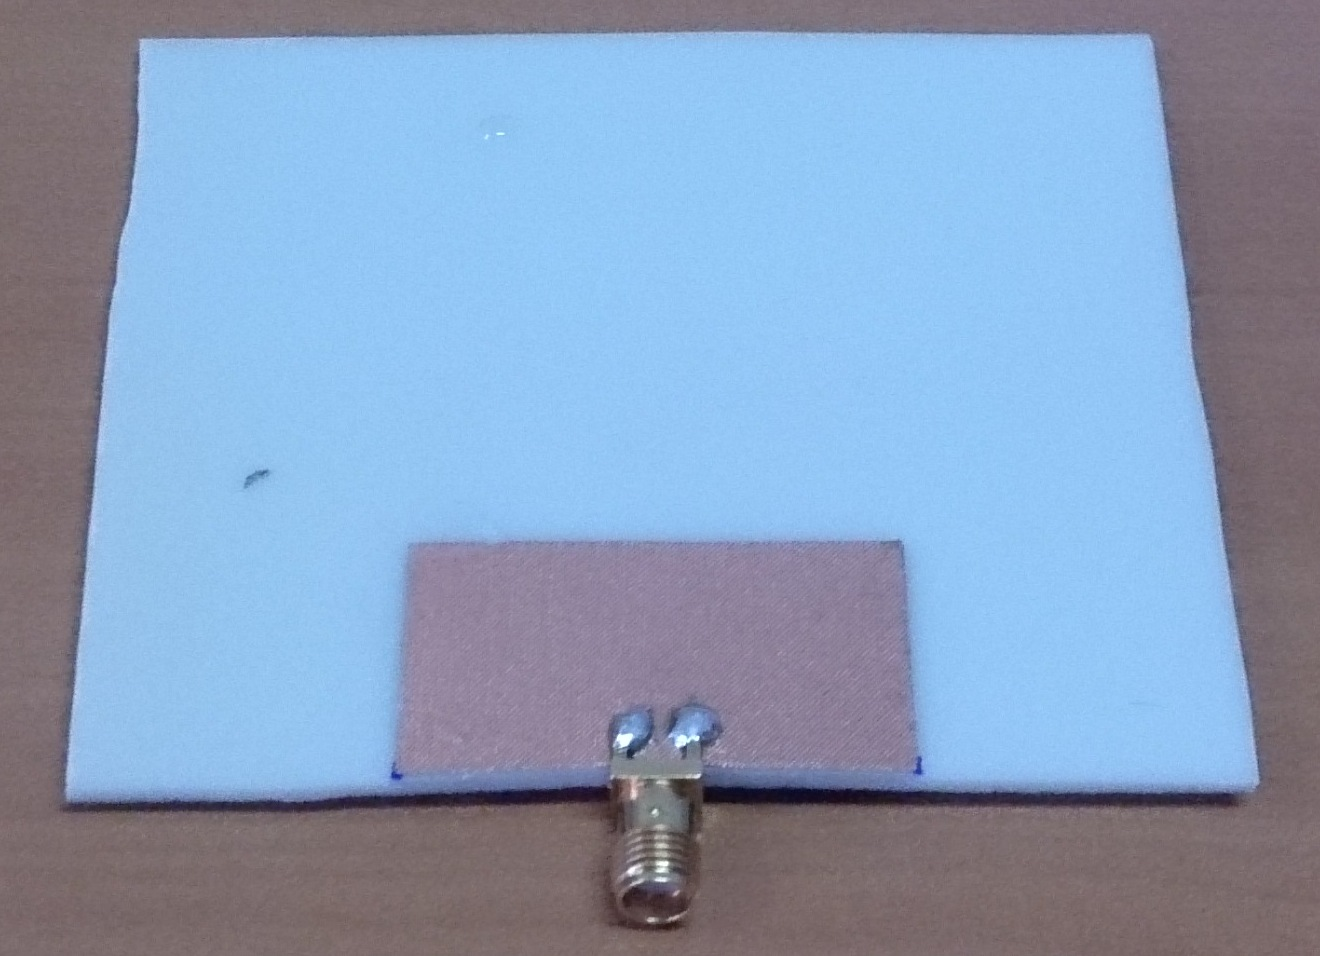
\includegraphics[width=\textwidth, height=0.75\textwidth]{images/patch_proto_back.jpg}
    \end{column}
    \end{columns}
  \end{frame}

\subsection{Metingen}
  \begin{frame}
  \frametitle{Metingen}

	  \begin{columns}[c]
	  \begin{column}{0.5\textwidth}
	  	\begin{itemize}
	  		\item Vergelijking met referentie
	  		\begin{itemize}
	  			\item Versie 1: $S_{11} > \SI{-10}{\decibel}$ 
	  		\end{itemize}
	  		\item Resonantie piek @ $\SI{5.2}{\giga\hertz}$  
	  		\begin{itemize}
	  			\item $\neq$ Simulatie
	  			\item Manuele fabricatie
	  			\item ADS: oneindig substraat
	  		\end{itemize}
	  	\end{itemize}
	  \end{column}%
	  \begin{column}{0.5\textwidth}
	  	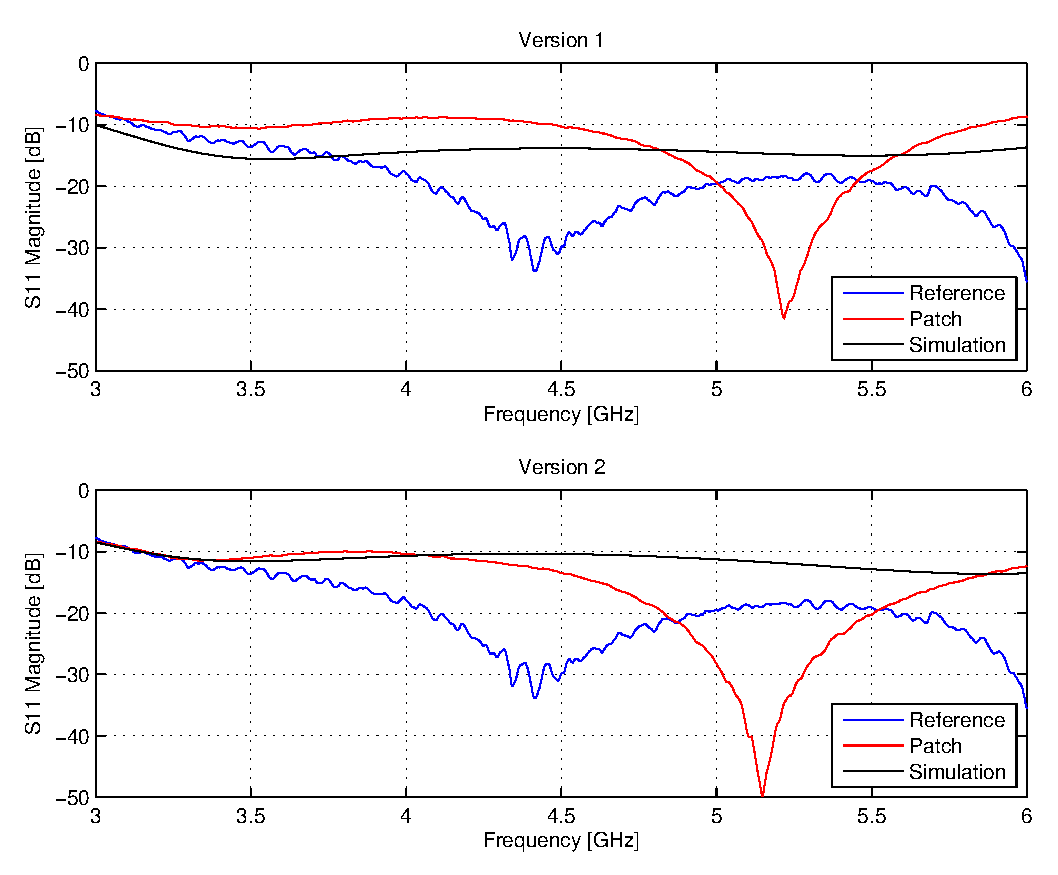
\includegraphics[width=\textwidth]{images/antenna_comparison}
	  \end{column}
	  \end{columns}
  \end{frame}

  \begin{frame}
  \frametitle{Metingen}
  	\begin{columns}[c]
  	\begin{column}{0.5\textwidth}
  		\begin{itemize}
  			\item Radiatiepatroon azimuth
  			\begin{itemize}
  				\item $\approx$ Omnidirectioneel tot $\SI{5}{\giga\hertz}$
  				\item Conform design parameters\\
  			\end{itemize}
  			\item Resonantie @ $\SI{5.2}{\giga\hertz}$
  			\begin{itemize}
  				\item Niet omni
  				\item Gain $\uparrow$
  			\end{itemize}
  			\item Transmit vermogen RCM instelbaar
  			\begin{itemize}
  				\item $[\SI{-31.6}{\decibel}m , \SI{-12.46}{\decibel}m]$
  			\end{itemize}
  		\end{itemize}
  	\end{column}
  	\begin{column}{0.5\textwidth}
  		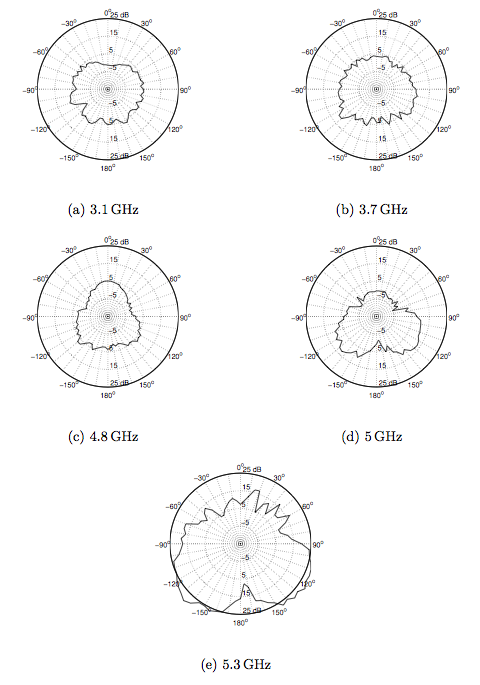
\includegraphics[width=0.8\textwidth]{images/ant_rad_pat.png}
  	\end{column}
  	\end{columns}
  \end{frame}

  \begin{frame}
  \frametitle{Metingen}
    \begin{columns}[c]
    \begin{column}{0.5\textwidth}
      \begin{itemize}
        \item Radiatiepatroon elevatie
        \begin{itemize}
          \item Twee nullen: \\ $\theta=0$ en $\theta=\pi$
          \item Drone recht boven anker: zeldzaam $\implies$ \hcancel{$\theta = 0$}
        \end{itemize}
      \end{itemize}
    \end{column}
    \begin{column}{0.5\textwidth}
      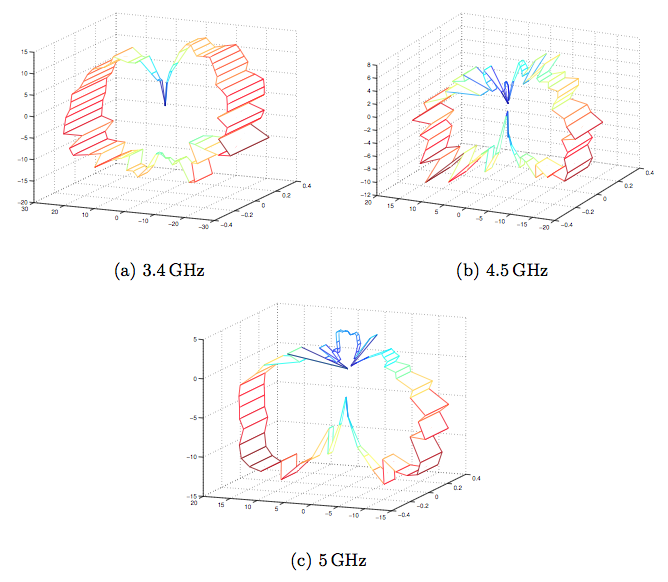
\includegraphics[width=\textwidth]{images/3D_rad_pat_ant.png}
    \end{column}
    \end{columns}
  \end{frame}

  \begin{frame}
  \frametitle{Metingen}
    \begin{columns}
    \begin{column}{0.5\textwidth}
      \begin{itemize}
        \item Plaatsing: Drone in nul 
        \begin{itemize}
          \item \hcancel{$\theta=\pi$}
          \item Risico EMC-problemen $\downarrow$
        \end{itemize}
      \end{itemize}
      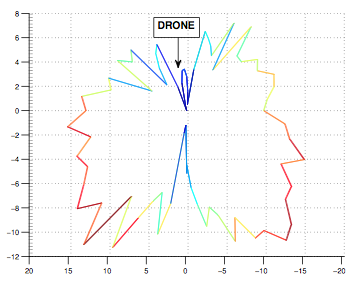
\includegraphics[width=0.9\textwidth]{images/mount_ant_drone.png}
    \end{column}
    \begin{column}{0.5\textwidth}
      \begin{itemize}
        \item Antenne effici\"entie
        \begin{itemize}
          \item Simulatie: $\frac{1}{exp(f)}$
          \item Tussen 10\% en 50\%
        \end{itemize}
      \end{itemize}
      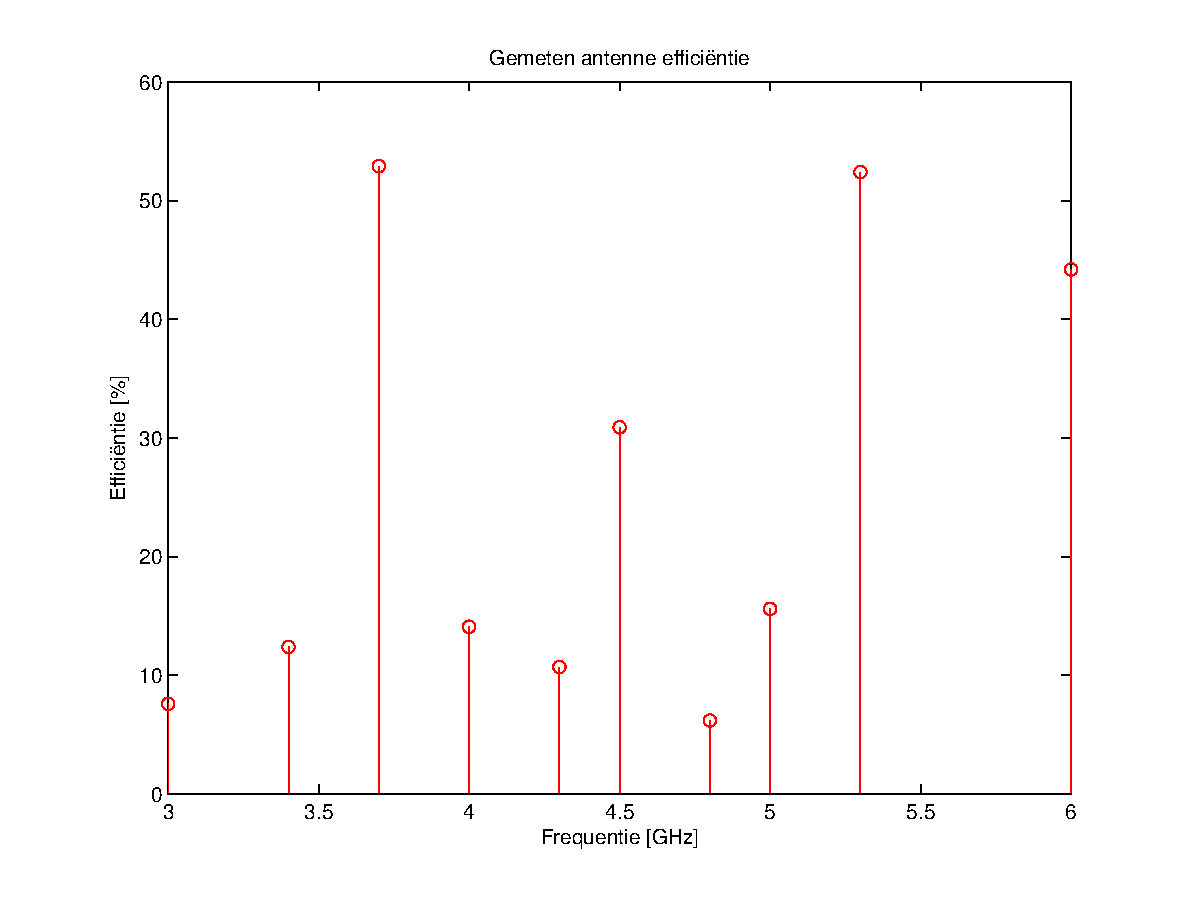
\includegraphics[width=\textwidth]{images/ant_eff}
    \end{column}
    \end{columns}
  \end{frame}

\subsection{Conclusie}
  \begin{frame}
  \frametitle{Conclusie Ontwerp Antenne}
    \begin{itemize}
      \item Antenne functioneert correct in systeem
      \item Openstaande problemen:
      \begin{itemize}
        \item Resonantie piek @ $\SI{5.2}{\giga\hertz}$ \\ $\implies$ Verbeter omnidirectionaliteit
        \item Antenne effici\"entie
        \item Aerodynamica
      \end{itemize}
    \end{itemize}

  \end{frame}

\section{Besluit}
  \begin{frame}
  \frametitle{Besluit}
    \begin{itemize}
      \item Antenne functioneert correct voor plaatsbepaling
      \item Algoritmes succesvol ge\"implementeerd op microcontroller
        \begin{itemize}
          \item Least Squares 3D
          \item Unscented Kalman Filter
        \end{itemize}
      \item PCB functioneert correct
      \item GUI aangepast
        \begin{itemize}
          \item Switchen tussen algoritmes
          \item Positie drone visueel voorstellen in 3D
          \item Accelerometer data plotten
        \end{itemize} 
      \item Volledig systeem kan gedemonstreerd worden
    \end{itemize}

  \end{frame}



\section{Demonstratie}
\begin{frame}[c]
  \begin{center}
    \Huge Demonstratie
  \end{center}
\end{frame}



\begin{frame}[label=FINAL_TOC]
  \begin{multicols}{2}
    \frametitle{Inhoudstafel}
    \tableofcontents[]
  \end{multicols}
\end{frame}
\end{document}
